\section{Preparación inicial}
\vspace{2mm}
Antes de configurar el cluster HPC, debe realizarse primero una configuración inicial en todas las máquinas. 
\subsection{Actualización de los sistemas}

\vspace{2mm}
Al inicio, Bolido y Centella se encontraban con un sistema Debian 8, por lo que se realizó la migración a Debian 10. La actualización se realizó manualmente, cambiando en el fichero /etc/apt/sources.list los repositorios a los correspondientes de la versión siguiente y forzando después una actualización. \newline

Para actualizar de Debian 8 a Debian 9 \cite{debian8:upgrade}, el fichero debe apuntar a los siguientes repositorios:

\begin{lstlisting}[language=bash]
    deb http://httpredir.debian.org/debian stretch main contrib non-free
    deb http://httpredir.debian.org/debian stretch-updates main contrib non-free
    deb http://security.debian.org stretch/updates main contrib non-free
\end{lstlisting} 
\vspace{2mm}

Similar es la migración de Debian 9 a Debian 10 \cite{debian9:upgrade}, donde el fichero debe apuntar a los siguientes repositorios:

\begin{lstlisting}[language=bash]
    deb http://deb.debian.org/debian debian buster main
    deb http://deb.debian.org/debian buster-updates main
    deb http://deb.debian.org/debian buster/updates main
\end{lstlisting} 
\vspace{2mm}

Finalmente, se fuerza la actualización con:

\begin{minted}
{bash}
    $ sudo apt-get update
    $ sudo apt-get upgrade
    $ sudo apt-get dist-upgrade
    $ sudo reboot
\end{minted}

Por último, con los siguientes comandos se comprueba si el sistema se actualizó correctamente (figura \ref{debian:hostname}) y se elimina las dependencias obsoletas que ya no son necesarias en el sistema.

\begin{lstlisting}[language=bash]
    $ hostnamectl
    $ sudo apt --purge autoremove
\end{lstlisting}

\begin{figure}[htb]
   \centering
   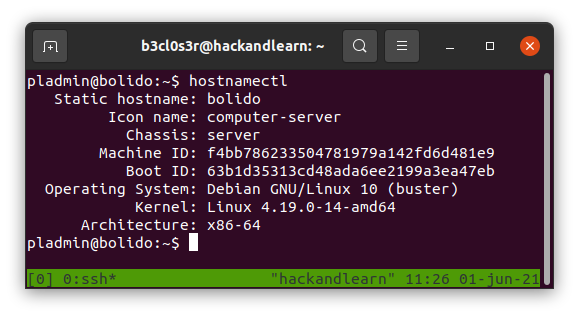
\includegraphics[width=0.9\linewidth]{images/hostnamectl.png}
   \caption{Comprobación de que el sistema se actualizó correctamente}
   \label{debian:hostname}
\end{figure}

\subsection{DNS}
\vspace{2mm}

Antes de configurar el \emph{cluster}, es conveniente que configuremos el DNS 
entre las tres máquinas. Para ello, solo hay que modificar el fichero /etc/hosts 
de cada máquina y añadir en cada línea dos pares separados por un espacio: dirección 
ip y los nombres que le asociaremos.
\vspace{2mm}

La configuración del fichero para las tres máquinas es como el siguiente:

\begin{lstlisting}[language=bash,caption={Fichero /etc/hosts},xleftmargin=.25\textwidth]

127.0.0.1	localhost 
192.168.1.2 bolido bolido.pcg.ull.es
192.168.1.3 rayo rayo.pcg.ull.es
192.168.1.4 centella centella.pcg.ull.es
\end{lstlisting}

\subsection{SSH}
\vspace{2mm}

SSH (Secure Shell) es un protocolo ampliamente utilizado para la gestión remota de máquinas. En nuestro caso, es necesario para poder acceder a nuestros ordenadores.
\vspace{2mm}


Para la instalación del cliente y servidor, se ejecutan los siguientes comandos respectivamente:
\vspace{2mm}

\begin{lstlisting}[language=bash]
    $ apt-get install openssh-client openssh-server
\end{lstlisting} 
\vspace{2mm}

Otro requisito para la creación del \emph{cluster}, es poder conectarse entre nodos realizando la autenticación sin contraseña. Para ello, como las carpetas de usuario se encuentran compartidas por NFS, se puede utilizar la autenticación mediante claves.
\vspace{2mm}

Para ello, se genera el par de claves automáticamente y se añade autoriza la clave pública:

\begin{lstlisting}[language=bash]
    $ ssh-keygen -t rsa
    $ cp ~/.ssh/id_rsa.pub authorized_keys
\end{lstlisting} 

\subsection{NTP}
\vspace{2mm}

Uno de los requisitos para poder configurar Slurm correctamente es que todos los ordenadores del \emph{cluster} tengan el reloj sincronizado. Para ello, hay que configurar NTP (Network Protocol Time), el protocolo que permite sincronizar los relojes de los ordenadores.
\vspace{4mm}

Se instala NTP en cada una de las máquinas con el siguiente comando:

\begin{lstlisting}[language=bash]
    $ apt-get install ntp
\end{lstlisting}
\vspace{4mm}

Tanto para configurar el cliente como el servidor, hay que modificar el fichero\newline /etc/ntp.conf.
\vspace{2mm}

En Bolido, se ha sincronizado su reloj con el pool de servidores oficial de Debian. Adicionalmente, se ha bloqueado acceso al servicio a todas las máquinas excepto a las pertenecientes al \emph{cluster} y un servidor de backup que mantenga la hora del sistema en caso de que la sincronización con los servidores externos falle. 
\vspace{4mm}

\begin{lstlisting}[language=bash,caption={Fichero /etc/ntp.conf de Bolido},xleftmargin=.25\textwidth]

# Backup server if official NTP servers fail
server  127.127.1.0
fudge   127.127.1.0 stratum 10

# Time servers
pool 0.debian.pool.ntp.org iburst
pool 1.debian.pool.ntp.org iburst
pool 2.debian.pool.ntp.org iburst
pool 3.debian.pool.ntp.org iburst

# Ignore all traffic
restrict default ignore
restrict -6 default ignore

# Allow localhost to manage ntpd
restrict 127.0.0.1
restrict ::1

# Allow servers to reply to our queries
restrict source nomodify noquery notrap

# Allow nodes to access ntp
restrict rayo nomodify
restrict centella nomodify
\end{lstlisting} 
\vspace{4mm}

En Rayo y Centella, se ha añadido a Bolido como servidor de referencia para sincronizar el reloj y se han comentado todos aquellos que hacían referencia a los oficiales de Debian.
\vspace{2mm}

\begin{lstlisting}[language=bash,caption={Fichero /etc/ntp.conf de Bolido},xleftmargin=.25\textwidth]

# ...

# Sincronizacion de reloj con Bolido
server bolido iburst

# ...

# Comentamos los servidores de debian 
# para que no se sincronice con ellos
# pool 0.debian.pool.ntp.org iburst
# pool 1.debian.pool.ntp.org iburst
# pool 2.debian.pool.ntp.org iburst
# pool 3.debian.pool.ntp.org iburst
\end{lstlisting}
\vspace{4mm}

Con el comando \lstinline[language=bash]!ntpq! se puede comprobar que los nodos tienen la hora sincronizada con bólido (figura \ref{ntp:checksync}).


\begin{figure}[htb]
   \centering
   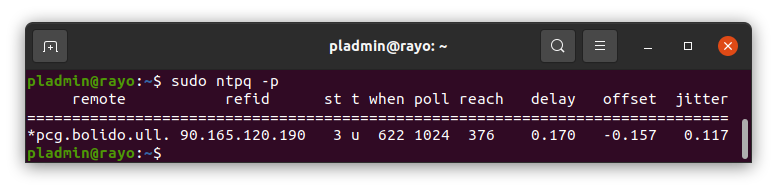
\includegraphics[width=0.9\linewidth]{images/ntpq-check.png}
   \caption{Comprobación de la sincronización del reloj}
   \label{ntp:checksync}
\end{figure}

\subsection{Munge}
\vspace{4mm}

Munge es un servicio de autenticación y validación de credenciales. Se utilizará con Slurm para validar sus procesos.
\vspace{2mm}

Para instalar y habilitar el servicio, se ejecuta:

\begin{lstlisting}[language=bash]
    $ apt-get install libmunge-dev libmunge2 munge
    $ systemctl enable munge
    $ systemctl start munge
\end{lstlisting}
\vspace{2mm}

En la figura \ref{munge:controllercheck} se comprueba que munge funciona correctamente, codificando y decodificando claves desde el controlador (Bolido).


\begin{figure}[htb]
   \centering
   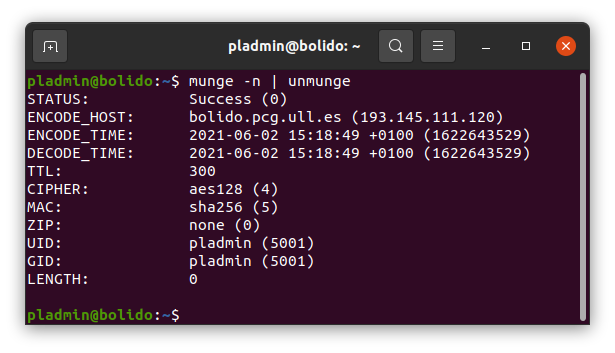
\includegraphics[width=0.8\linewidth]{images/mungecontroller.png}
   \caption{Comprobación codificación y decodificación de claves de Munge en el controlador}
   \label{munge:controllercheck}
\end{figure}
\vspace{2mm}

A continuación, en los nodos (Rayo y Centella) se copia la clave de la máquina principal (Bolido) y se guarda en /etc/munge con el usuario munge de propietario y con permiso de lectura únicamente para este usuario.

\vspace{2mm}

\begin{lstlisting}[language=bash]
    $ scp bolido:/etc/munge/munge.key /etc/munge/
    $ chown munge:munge /etc/munge/munge.key
    $ chmod 400 /etc/munge/munge.key
\end{lstlisting}
\vspace{2mm}

En la figura \ref{munge:nodecheck}, se comprueba que munge funciona correctamente entre un nodo y el controlador: codificando desde un nodo y decodificando el hash generado desde el controlador.

\begin{figure}[htb]
   \centering
   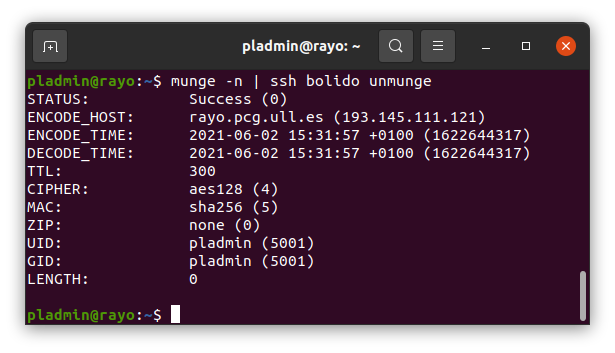
\includegraphics[width=0.8\linewidth]{images/mungenode.png}
   \caption{Comprobación codificación de clave de Munge en el nodo y decodificación en el controlador}
   \label{munge:nodecheck}
\end{figure}

\subsection{Creación de usuarios locales}
\vspace{4mm}

En todas las máquinas, se creó un usuario local común como administrador y un usuario llamado slurm con el mismo UID y GUID para el servicio de Slurm. 
\vspace{4mm}

Se empleó los siguientes comandos: 

\begin{lstlisting}[language=bash]
    groupadd -g 5000 slurm
    useradd slurm -u 5000 -g 5000 
\end{lstlisting}

\section{Configuración del controlador}

El controlador (Bolido) es la máquina de entrada del \emph{cluster}. Se encarga de administrar, gestionar los recursos, ejecutar tareas sobre los nodos y proveer de autenticación centralizada y de software y herramientas a los nodos.

\subsection{NFS}

NFS \cite{nfs} (Network File System) es un protocolo de nivel de aplicación utilizado para compartir sistemas de archivos entre ordenadores. En nuestro \emph{cluster}, permite centralizar el software que proveeremos y las carpetas personales de los usuarios en todo el sistema.
\vspace{4mm}

El paquete se instala con:
\begin{lstlisting}[language=bash]
    $ apt-get install nfs-kernel-server 
\end{lstlisting}
\vspace{4mm}

A continuación, se modifica el fichero /etc/exports para compartir los directorios de /home y /opt con permisos de escritura y mapeo de root independientemente del sistema (no\_root\_squash).
\vspace{2mm}

\begin{lstlisting}[language=bash,caption={Fichero /etc/exports de Bolido}]

/home	rayo(rw,sync,no_root_squash,no_subtree_check)
        centella(rw,sync,no_root_squash,no_subtree_check)
        
/opt	rayo(rw,sync,no_root_squash,no_subtree_check)
        centella(rw,sync,no_root_squash,no_subtree_check)
\end{lstlisting}

%%%% CONFIGURACION LDAP SERVIDOR %%%%
\subsection{LDAP}

LDAP (Lightweight Directory Access Protocol) \cite{ldap} es un protocolo de nivel de aplicación que permite el acceso a servicio de directorio de forma ordenada y distribuida. En concreto, se utilizará para compartir a los nodos los usuarios y grupos que existen en nuestro sistema.

\vspace{2mm}
Se instala LDAP como servidor con la siguiente instrucción:
\vspace{2mm}

\begin{lstlisting}[language=bash]
    $ apt-get install slapd
\end{lstlisting}
\vspace{2mm}

A continuación, se reconfigura LDAP:
\vspace{2mm}

\begin{lstlisting}[language=bash]
    $ sudo dpkg-reconfigure slapd
\end{lstlisting}
\vspace{2mm}
En él, se establece como nombre distinguido (DN) base dc=bolido,dc=pcg,dc=ull,dc=es y se crea una nueva base de datos con su usuario de administrador.
\vspace{2mm}

Para que el sistema local autentique los usuarios contra LDAP, se debe instalar los siguientes paquetes:

\vspace{2mm}
\begin{lstlisting}[language=bash]
    $ sudo apt-get install libnss-ldapd nscd nslcd
\end{lstlisting}
\vspace{2mm}

Durante la instalación, aparecerán una serie de pantallas para configurar LDAP. Se debe establecer en ella la dirección IP del LDAP del servidor (Bolido), el nombre distinguido para la base de las busquedas (dc=bolido, dc=pcg, dc=ull, dc=es), la versión de LDAP (3) y el usuario administrador de LDAP. Esto configurará nscd y nslcd con sus respectivos ficheros de configuración: libnss-ldap.conf y nslcd.conf.
\vspace{2mm}

Es importante que se instale libnss-ldapd en lugar de libnss-ldap. Esta versión es una mejora que ofrece mejor depuración, mejor rendimiento y separación del código de NSS, LDAP y PAM \cite{libnsspamd}. 
\vspace{2mm}

Por último, hay que indicar en el fichero /etc/nsswitch.conf que emplee LDAP como servicio de autenticación.
\vspace{2mm}
\begin{lstlisting}[language=bash,caption={Fichero /etc/nsswitch.conf},xleftmargin=.25\textwidth]
passwd:         files ldap systemd 
group:          files ldap systemd
shadow:         files ldap
gshadow:        files ldap

\end{lstlisting}
\vspace{2mm}

Es importante que LDAP se encuentre antes que systemd para que al realizar la autenticación, el sistema intente rescatar primero la información de las bases de datos, después de LDAP y, en caso de no lograrlo, pregunte a los demonios del sistema.
\vspace{2mm}

Para gestionar LDAP, se puede utilizar ldap-utils, ldapvi y cpu. Ldap-utils provee de herramientas para manipular las bases de datos, LDAPvi permite modificar LDAP como si se utilizara un editor de texto y CPU facilita las tareas de añadir nuevos usuarios y grupos al sistema.

\vspace{2mm}
\begin{lstlisting}[language=bash]
    $ apt-get install ldap-utils cpu ldapvi
\end{lstlisting}
\vspace{2mm}

En primer lugar, es conveniente configurar el fichero ldap.conf, el fichero de configuración para las herramientas de cliente de LDAP. Este debe tener permisos de lectura y escritura solo para root, para evitar fallos de seguridad.

\begin{lstlisting}[language=bash,caption={Fichero /etc/ldap/ldap.conf},xleftmargin=.25\textwidth]
uri ldap://0.0.0.0
base dc=bolido,dc=pcg,dc=ull,dc=es
ldap_version 3
ssl start_tls
binddn cn=admin,dc=bolido,dc=pcg,dc=ull,dc=es
bindpw asafepasswordgoeshere
TLS_CACERT /etc/ssl/certs/ca-certificates.crt
\end{lstlisting}
\vspace{2mm}

A continuación, con el siguiente comando y fichero en formato ldif, se crean las unidades organizativas en las que se encontrarán los usuarios y grupos del \emph{cluster}.

\vspace{4mm}
\begin{lstlisting}[language=bash]
    $  ldapadd -x -D "cn=admin,dc=bolido,dc=pcg,dc=ull,dc=es" 
       -W -H ldap:// -f userandgroups.ldif
\end{lstlisting}
\vspace{2mm}

\vspace{2mm}
\begin{lstlisting}[language=bash,caption={fichero userandgroups.ldif}]
    dn: ou=People,dc=bolido,dc=pcg,dc=ull,dc=es
    objectClass: organizationalUnit
    description: bolido users and groups
    ou: People
    
    dn: ou=Users,ou=People,dc=bolido,dc=pcg,dc=ull,dc=es
    objectClass: organizationalUnit
    description: bolido users
    ou: Users
    
    dn: ou=Groups,ou=People,dc=bolido,dc=pcg,dc=ull,dc=es
    objectClass: organizationalUnit
    description: bolido groups
    ou: Groups
\end{lstlisting}
\vspace{4mm}

Ahora, se configura la herramienta CPU \cite{ldapcpu} para que cree de una forma más sencilla los usuarios en LDAP. Para ello, primero se debe configurar el fichero /etc/cpu/cpu.conf y establecer la opción de SHADOWLASTCHANGE a 0 para forzar que cuando el usuario se conecte deba que cambiar la contraseña.

\vspace{4mm}
\begin{lstlisting}[language=bash,caption={fichero /etc/cpu/cpu.conf}]
# ...
LDAP_URI    = ldap://localhost
BIND_DN     = cn=admin,dc=bolido,dc=pcg,dc=ull,dc=es
BIND_PASS   = password
USER_BASE   = ou=Users,ou=People,dc=bolido,dc=pcg,dc=ull,dc=es
GROUP_BASE  = ou=Groups,ou=People,dc=bolido,dc=pcg,dc=ull,dc=es
# ...
SHADOWLASTCHANGE = 0
\end{lstlisting}
\vspace{4mm}

Ahora, es posible crear y eliminar usuarios dentro de nuestro \emph{cluster} de una forma muy sencilla:

\vspace{6mm}
\begin{lstlisting}[language=bash]
    $ cpu useradd $USERNAME -m  -p$PASSWORD
    $ cpu userdel -r $USERNAME
    $ cpu groupdel $USERNAME
\end{lstlisting}
\vspace{4mm}

Con la opción -m, CPU crea el directorio home del usuario. Para eliminar usuarios, se utiliza -r para eliminar también su directorio \emph{home}. Por defecto, CPU crea el grupo del usuario pero no lo elimina, por lo que hay que hacerlo manualmente.
\vspace{4mm}

Con LDAPvi \cite{ldapvi}, se puede modificar LDAP con un editor de texto utilizando el siguiente comando:

\begin{lstlisting}[language=bash]
    $ ldapvi -D  "cn=admin,dc=bolido,dc=pcg,dc=ull,dc=es"
\end{lstlisting}

\subsection{Slurm}

Slurm \cite{slurmquickstart} es un sistema de gestión de sistemas y de clústeres, y está compuesto por distintas herramientas y servicios.
\vspace{4mm}

Dentro de los servicios, existen: 
\vspace{2mm}
\begin{itemize}
    \item \textbf{Slurmctld: } controlador del \emph{cluster}. 
    \item \textbf{Slurmd: } demonio de los nodos del \emph{cluster}.
    \item \textbf{Slurmdbd: } interfaz para interacturar con la base de datos de Slurm. No se configurará porque para el uso de este \emph{cluster} no aporta ninguna funcionalidad útil.
\end{itemize}
\vspace{4mm}

El cliente puede hacer uso de los siguientes comandos:
\vspace{2mm}

\begin{itemize}
    \item \textbf{sacct: } informa de trabajos activos o completados.
    
    \item \textbf{salloc: } reserva recursos para un trabajo.
    
    \item \textbf{sttach: } permite vincularse a las entradas y salidas de un trabajo en ejecución.
    
    \item \textbf{sbatch: } utilidad para enviar un script como trabajo.
    
    \item \textbf{sbcast: } transfiere un fichero desde el disco local a un nodo.
    
    \item \textbf{scancel: } cancelar tareas pendientes o en ejecución. 

    \item \textbf{scontrol: } es una herramienta administrativa utilizada para ver o modificar el estado de Slurm.
    
    \item \textbf{sinfo: } muestra el estado de las particiones y nodos gestionados por slurm.

    \item \textbf{sprio: } muestra información detallada de los componentes que afectan a la prioridad de un trabajo.

    \item \textbf{squeue: } muestra información sobre el estado de los trabajos.

    \item \textbf{srun: } permite lanzar trabajos para ejecutar.

    \item \textbf{sshare: } muestra información detallada sobre el uso del \emph{cluster}.

    \item \textbf{sstat: } obtiene información sobre los recursos utilizados por un trabajo.

    \item \textbf{strigger: } permite establecer, obtener o observar cuándo ocurre un evento, como trabajos que han alcanzado el tiempo límite.
    
    \item \textbf{sview: } interfaz gráfica que obtiene información del estado para trabajos, particiones y nodos gestionados por Slurm. \newline
\end{itemize}

\begin{figure}[htb]
   \centering
   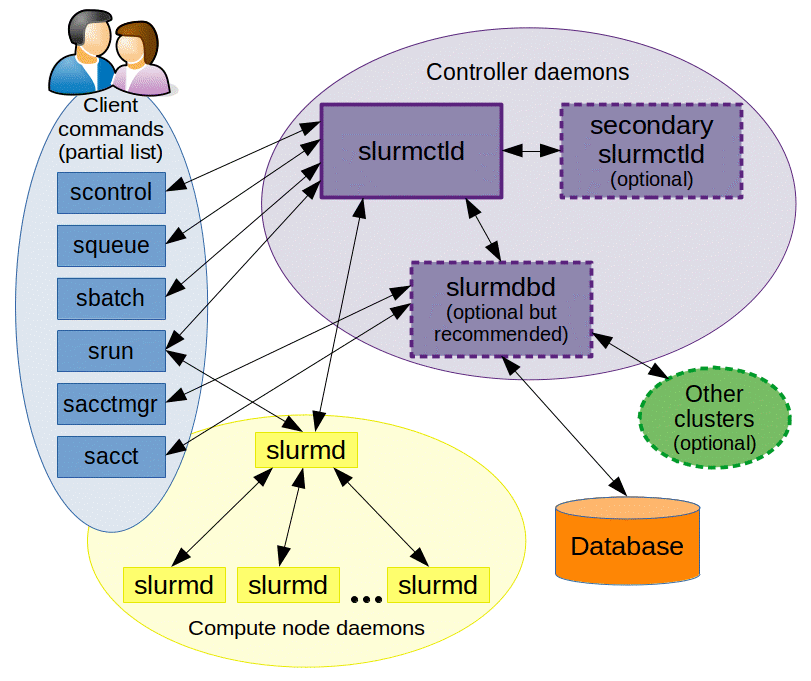
\includegraphics[scale=0.3]{images/slurmcomponents.png}
   \caption{Componentes de slurm}
   \label{nfs:server}
\end{figure}
\vspace{4mm}
Instalamos slurm en el servidor con:
\vspace{2mm}
\begin{lstlisting}[language=bash]
    $ apt-get install slurm-wlm slurm-client
\end{lstlisting}
\vspace{2mm}
Como slurmd no es necesario en el controlador, se puede desactivar el demonio con:
\vspace{2mm}
\begin{lstlisting}[language=bash]
    $ systemctl stop slurmd
    $ systemctl disable slurmd
\end{lstlisting}
\vspace{2mm}

Para configurar Slurm (/etc/slurm-llnl/slurm.conf), se ha generado el fichero de configuración desde el generador de la documentación oficial \cite{slurmconfiguration}.
\vspace{4mm}

Al final de este fichero, se ha incluido la información de los nodos que componen el cluster y se han creado 3 colas para lanzar trabajos.
\vspace{2mm}

%%% CAMBIAR %%%
\vspace{2mm}
\begin{lstlisting}[language=bash,caption={Fichero /etc/slurm-llnl/slurm.conf}]
NodeName=rayo CPUs=48 Boards=1 SocketsPerBoard=4 CoresPerSocket=12 
ThreadsPerCore=1 RealMemory=64408
NodeName=centella CPUs=48 Boards=1 SocketsPerBoard=8 CoresPerSocket=6 
ThreadsPerCore=1 RealMemory=64392

PartitionName=rayo Nodes=rayo MaxTime=INFINITE State=UP
PartitionName=centella Nodes=centella MaxTime=INFINITE State=UP
PartitionName=short Nodes=rayo,centella Default=YES MaxTime=INFINITE State=UP
\end{lstlisting}
\vspace{2mm}

\subsection{Lmod}
\vspace{2mm}

Lmod \cite{lmod} es una herramienta que permite personalizar las variables de entorno del usuario. Dentro del cluster, será útil para poder cargar distintas herramientas y poder utilizar distintas versiones de una misma, evitando problemas a la hora de trabajar con dependencias y facilitando la gestión del entorno.
\vspace{4mm}

Primero hay que instalar Lua \cite{lmod}. Para ello, se descarga la última versión y se almacena en /opt/storage/downloads.

\vspace{2mm}
\begin{lstlisting}[language=bash]
  $ wget https://sourceforge.net/projects/lmod/files/lua-5.1.4.9.tar.bz2
\end{lstlisting}
\vspace{2mm}

A continuación, se instala lua en /opt/soft con su versión correspondiente y se debe crear el enlace simbólico al binario en el sistema.
\vspace{2mm}

\begin{lstlisting}[language=bash]
    $ tar xf lua-5.1.4.9.tar.bz2
    $ cd lua-X.Y.Z
    $ ./configure --prefix=/opt/soft/lua/5.1.4.9
    $ make; make install
    $ cd /opt/soft/lua; ln -s 5.1.4.9 lua
    $ mkdir /usr/local/bin; ln -s /opt/soft/lua/5.1.4.9/lua/bin/lua /usr/local/bin
\end{lstlisting}
\vspace{2mm}

Para instalar lmod, se debe crear la carpeta /opt/soft/lmod/, clonar el repositorio oficial y compilarlo:

\vspace{2mm}
\begin{lstlisting}[language=bash]
  $ git clone https://github.com/TACC/Lmod
  $ cd lmod
  $ ./configure --prefix=/opt/soft
  $ make install
\end{lstlisting}
\vspace{2mm}

A continuación, hay que crear un enlace simbólico con el script generado por lmod y vincularlo con el /etc/profile.d del sistema, para que cuando un usuario ejecute una terminal se inicialicen las variables de entorno de lmod.

\vspace{2mm}
\begin{lstlisting}[language=bash]
ln -s /opt/apps/lmod/lmod/init/profile        /etc/profile.d/z00_lmod.sh
\end{lstlisting}
\vspace{2mm}

Finalmente, se puede comprobar si lmod está correctamente instalando comprobando su variable de entorno:

\vspace{2mm}
\begin{lstlisting}[language=bash]
    $ echo $MODULEPATH
\end{lstlisting}
\vspace{2mm}

Para proveer de herramientas a los usuarios, se deben crear unos ficheros llamados modulefiles, en los que se indican como debe modificarse las variables del entorno del sistema (frecuentemente, \$PATH y \$LD\_LIBRARY\_PATH).
\vspace{2mm}

La organización para los programas que se ha utilizado es la siguiente. Primero, se ha creado el directorio /opt/soft/modulefiles/Linux e, internamente, una carpeta para cada herramienta. Dentro de cada herramienta, se crea un fichero .lua cuyo nombre es la versión que carga de esa herramienta, permitiendo así tener distintas versiones de un mismo programa o librería.
\vspace{4mm}

Algunos comandos básicos para utilizar lmod son los siguientes:
\vspace{4mm}

- Mostrar el software disponible:
\vspace{2mm}
\begin{lstlisting}[language=bash]
    $ module spider
\end{lstlisting}
\vspace{4mm}

- Cargar en el entorno software concreto:
\vspace{2mm}
\begin{lstlisting}[language=bash]
    $ module load name/version
\end{lstlisting}
\vspace{4mm}

- Mostrar modulefile de un software concreto:
\vspace{2mm}
\begin{lstlisting}[language=bash]
    $ module show name/version
\end{lstlisting}


\subsection{Quota}

Para evitar el consumo excesivo de espacio de disco por parte de los usuarios, se ha limitado utilizando quota.

\vspace{2mm}
\begin{lstlisting}[language=bash]
    $ apt-get install quota
\end{lstlisting}
\vspace{2mm}

Hay que modificar el fichero /etc/fstab, añadiendo que se van a utilizar las quotas de usuario sobre la partición /home.
\vspace{4mm}

\begin{lstlisting}[language=bash, caption={Configuración /etc/fstab en Bolido para Quotas}]
# ...
/dev/mapper/bolido--home-home /home ext4 defaults,usrquota   0  2
# ...
\end{lstlisting}
\vspace{4mm}

A continuación, se activan las quotas de usuario en /home con el siguiente comando:

\vspace{2mm}
\begin{lstlisting}[language=bash]
    $ quotaon -uv /home
\end{lstlisting}
\vspace{2mm}

Para facilitar la creación de usuarios y la asignación de quotas, se creó un script para el administrador de sistemas.

\subsection{Script de gestión de usuarios}

Para facilitar la gestión de usuarios dentro del \emph{cluster}, se programó una pequeña herramienta en bash con la que crear los usuarios en LDAP y asignarles automáticamente las quotas (ver apéndice 1). 
\vspace{4mm}

La herramienta se encuentra guarda en /usr/local/sbin para que solo esté disponible para root bajo el nombre de cluster-user-management.
\vspace{4mm} 

Ejemplos de uso:
\vspace{4mm} 

Crear usuario test con contraseña testbolido y asignar 25G de quota de disco:
\begin{lstlisting}[language=bash]
    $  ./cluster-user-management -a test -q 25G
\end{lstlisting}
\vspace{4mm} 

Modificar las quotas de disco del usuario test a 500 megas:

\begin{lstlisting}[language=bash]
    $ ./cluster-user-management -m test -q 500M
\end{lstlisting}
\vspace{4mm} 

Eliminar usuario test:
\begin{lstlisting}[language=bash]
    $ ./cluster-user-management -d test
\end{lstlisting}
 
\section{Configuración de los nodos}
\subsection{NFS}

Autofs permite montar sistemas de archivos bajo demanda. Esto es especialmente útil para los nodos del cluster. 
\vspace{2mm}

Se instala autofs con:
\vspace{2mm}
\begin{lstlisting}[language=bash]
    $ apt-get install autofs
\end{lstlisting}
\vspace{4mm}
Después, hay que crear el fichero /etc/auto.master, en el que añade al final del fichero la ruta local de montaje y el fichero de referencia:

\vspace{4mm}
\begin{lstlisting}[language=bash]
    /home   /etc/auto.home
    /opt    /etc/auto.opt
\end{lstlisting}
\vspace{4mm}

A continuación, se crea el fichero /etc/auto.home con:

\begin{lstlisting}[language=bash]
    * -fstype=nfs4  bolido:/home/&
\end{lstlisting}
\vspace{4mm}

Y un fichero /etc/auto.opt con:

\vspace{2mm}
\begin{lstlisting}[language=bash]
    * -fstype=nfs4  bolido:/opt/&
\end{lstlisting}
\vspace{2mm}

En ambos casos, se especifica que se monte utilizando nfs4 todo el contenido de las carpetas /home y /opt, incluyendo subdirectorios de estos.

%%% CONFIGURACION LDAP CLIENTE %%%

\subsection{LDAP}

Se instala LDAP en el cliente \cite{ldapconfiguration} con:
\vspace{2mm}

\begin{lstlisting}[language=bash]
    $ sudo apt-get install libnss-ldapd nscd nslcd
\end{lstlisting}
\vspace{2mm}

Se realiza la misma configuración que en el servidor, configurando nscd y nslcd. 

\vspace{2mm}
\vspace{4mm}

Es importante que se instale libnss-ldapd en lugar de libnss-ldap. Esta versión es una mejora que ofrece mejor depuración, mejor rendimiento y separación del código de NSS, LDAP y PAM \cite{libnsspamd}. 

\vspace{4mm}
Por último, se debe indicar en el fichero /etc/nsswitch.conf \cite{nsswitchconf} (fichero de configuración de la base de datos del sistema) para que utilice LDAP como servicio de autenticación.

\vspace{4mm}
\begin{lstlisting}[language=bash,caption={Fichero /etc/nsswitch.conf},xleftmargin=.25\textwidth]
passwd:         files ldap systemd 
group:          files ldap systemd
shadow:         files ldap
gshadow:        files ldap
\end{lstlisting}
\vspace{2mm}

Es importante que LDAP se coloque antes que systemd para que al realizar la autenticación, el sistema intente primero rescatar la información de las bases de datos, después de LDAP y, en caso de no lograrlo, pregunte a los demonios del sistema.

\vspace{2mm}
Se puede comprobar que el servicio está funcionando correctamente si el siguiente comando nos devuelve la información del /etc/passwd de LDAP:
\vspace{2mm}
\begin{lstlisting}[language=bash]
    $ getent passwd
\end{lstlisting}

\subsection{Slurm}

Se instala slurm en el cliente con:

\begin{lstlisting}[language=bash]
    $ apt-get install slurm-wlm
\end{lstlisting}
\vspace{2mm}

Se debe copiar el fichero de configuración que se encuentra en Bolido y guardarlo en /etc/slurm-llnl bajo el nombre de slurm.conf. También se debe generar una clave privada y un certificado para el nodo.
\vspace{4mm}

\begin{lstlisting}[language=bash]
$ openssl genrsa -out /etc/slurm-llnl/slurm.key 1024
$ openssl rsa -in /etc/slurm-llnl/slurm.key -pubout 
  -out /etc/slurm-llnl/slurm.cert
\end{lstlisting}
\vspace{4mm}

Con el siguiente comando, se puede generar la información sobre el nodo para incluirlo en el fichero de configuración de slurm:

\vspace{2mm}
\begin{lstlisting}[language=bash]
    $ slurmd -C
\end{lstlisting}

\subsection{Bloqueo de autenticación de usuarios}
\vspace{2mm}

Se puede evitar que los usuarios no puedan conectarse por SSH a los nodos, manteniendo la posibilidad de que lancen trabajos con slurm. Para ello, hay que instalar libpam-slurm y modificar cómo se realiza la autenticación de SSH a través de las PAM.

\vspace{2mm}
\begin{lstlisting}[language=bash]
    $ apt-get install libpam-slurm
\end{lstlisting}
\vspace{2mm}

Por último, se modificó el fichero /etc/pam.d/sshd. Se añadió la siguiente línea para permitir autenticación local para el usuario de administración: 

\vspace{2mm}
\begin{lstlisting}[language=bash]
    $ account    sufficient   pam_localuser.so
\end{lstlisting}
\vspace{2mm}

De acuerdo a la documentacion \cite{slurmpam}, se añadió también esta línea como última opción de las cuentas, para bloquear a todos los usuarios que no tengan una instancia de slurm en la máquina:
 
\vspace{2mm}
\begin{lstlisting}[language=bash]
    $ account    required      pam_slurm_adopt.so
\end{lstlisting}
\vspace{2mm}



\section{Instalación de herramientas}

Todas las herramientas que se proveen dentro del cluster se encuentran compartidas por NFS en el directorio /opt/soft y los usuarios del cluster pueden cargarlas y seleccionar entre distintas versiones disponibles gracias a lmod.

\subsection{OpenMPI}

OpenMPI es una implementación del estándar MPI \cite{mpi} (Interfaz de Paso Mensajes), que define la sintáxis y la semántica de las funciones que deben encontrarse en una librería de pasos de mensajes para ser utilizada por programas que aprovechan la existencia de distintos procesadores.
\vspace{2mm}

Para instalar OpenMPI, primero hay que descargarlo del directorio oficial:

\vspace{4mm}

\begin{lstlisting}[language=bash]
    $ wget https://download.open-mpi.org/release/open-mpi
           /v3.1/openmpi-3.1.6.tar.gz
\end{lstlisting}
\vspace{4mm}

A continuación, se crean los directorios donde se almacenará OpenMPI, se instala en el sistema varias librerías necesarias para que openmpi y slurm funcionen correctamente, y se configura y compila OpenMPI.

\vspace{4mm}
\begin{lstlisting}[language=bash]
    $ mkdir -p /opt/soft/openmpi/3.1.6
    $ sudo apt-get install -y libpmi2-0-dev libpmi2-0
    $ ./configure --prefix=/opt/soft/openmpi/3.1.6  --with-slurm --with-pmi           --with-pmi-libdir=/usr/lib/x86_64-linux-gnu
    $ make install all
\end{lstlisting}
\vspace{4mm}

Por último, se crea el modulefile para OpenMPI, en el que se incluyen los binarios a la variable PATH del sistema y las librerías dinámicas a la variable LD\_LIBRARY\_PATH.
\vspace{4mm}

\begin{lstlisting}[language=bash,caption={Modulefile de OpenMPI},xleftmargin=.15\textwidth]
help([[
For detailed instructions, go to:
   https://www.open-mpi.org/
]])
whatis("Version: 3.1.6")
whatis("Keywords: Compiler OpenMPI")

setenv("OPENMPIPATH", "/opt/soft/openmpi/3.1.6/bin")
prepend_path( "PATH", "/opt/soft/openmpi/3.1.6/bin")
prepend_path( "LD_LIBRARY_PATH","/opt/soft/openmpi/3.1.6/lib")
\end{lstlisting}
\vspace{4mm}

Se realiza el proceso equivalente para instalar la versión 4.1.1.

\subsection{OpenBLAS}

OpenBLAS \cite{openblas} es una implementación open source de las API de BLAS (Basic Linear Algebra Subprograms) y LAPACK con distintas optimizaciones realizadas manualmente para distintos tipos de procesador.
\vspace{2mm}

Se descarga y compila OpenBLAS con:

\vspace{4mm}
\begin{lstlisting}[language=bash]
$ git clone https://github.com/xianyi/OpenBLAS.git
$ mv OpenBLAS /opt/soft/openblas/3.14
$ make
\end{lstlisting}
\vspace{4mm}

OpenBLAS solo se puede utilizar como librería estática o dinámica, por lo que solo se necesita poner a disposición del usuario los ficheros generados que se encuentran en lib mediante la variable de entorno LD\_LIBRARY\_PATH.
\vspace{2mm}
\begin{lstlisting}[language=bash,caption={Modulefile de OpenBLAS},xleftmargin=.15\textwidth]
help([[
For detailed instructions, go to:
   https://github.com/xianyi/OpenBLAS
]])
whatis("Version: 3.14")
whatis("Keywords: OpenBLAS")

prepend_path( "LD_LIBRARY_PATH","/opt/soft/openblas/3.14/lib")
\end{lstlisting}
\vspace{4mm}

\subsection{GSL}
GNU Scientific Library \cite{gsl} (GSL) es una librería numérica para programadores de C / C++.
\vspace{4mm}

Para instalar GSL, se descarga el paquete, se configura la carpeta de salida y se compila con las siguientes instrucciones:

\begin{lstlisting}[language=bash]
$ wget https://mirrors.up.pt/pub/gnu/gsl/gsl-latest.tar.gz
$ tar xf gsl-lastest.tar.gz
$ ./configure --prefix=/opt/soft/gsl/2.7
$ make install
\end{lstlisting}
\vspace{4mm}

Por último, se genera el modulefile para poner a disposición de los usuarios la librería:
\vspace{4mm}

\begin{lstlisting}[language=bash,caption={Modulefile de GSL},xleftmargin=.15\textwidth]
help([[
For detailed instructions, go to:
   https://www.gnu.org/software/gsl/
]])
whatis("Version: 2.7")
whatis("Keywords: Compiler GSL")

prepend_path( "PATH", "/opt/soft/gsl/2.7/bin")
prepend_path( "LD_LIBRARY_PATH","/opt/soft/gsl/2.7/lib")
\end{lstlisting}
\vspace{4mm}

\subsection{Intel Performance Tools}

Intel provee de un conjunto de herramientas para computación de alto rendimiento: compiladores, librerías y herramientas para análisis, depuración y tuneado.
\vspace{2mm}

Para instalar OneApi, se añadió el repositorio de intel a apt y se descargó el paquete de OneApi \cite{inteloneapi} y, con todos los paquetes descargados, se instalaron individualmente en el directorio /opt/soft.
\vspace{2mm}

\begin{lstlisting}[language=bash]
    $ wget https://apt.repos.intel.com/intel-gpg-keys/
      GPG-PUB-KEY-INTEL-SW-PRODUCTS.PUB -O - |
      sudo apt-key add -
    $ echo "deb https://apt.repos.intel.com/oneapi all main" | 
      sudo tee /etc/apt/sources.list.d/oneAPI.list
    $ sudo apt install intel-basekit
    $ cd /var/cache/apt/archives
    $ packages = $(ls intel*.deb)
    $ for i in ${packages[@]}; do 
        dpkg-deb -x $i /opt/soft/intel/oneapi/; 
      done
\end{lstlisting}
\vspace{2mm}

Las herramientas de intel proveen de un script que genera automáticamente los modulefiles configurados.
\vspace{2mm}

Simplemente, se ejecutó el script y se copiaron todos los ficheros generados en nuestro directorio de modulefiles.
\vspace{2mm}

\begin{lstlisting}[language=bash]
    $ ./modulefiles-setup.sh
    $ mv modulefiles /opt/soft/modulefiles/Linux/oneapi
\end{lstlisting}


\section{Problemas}

En este apartado se comentan algunas de las dificultades encontradas a la hora de configurar el cluster.
\vspace{2mm}

\subsection{Configuración de Bolido en Raid 1}
En una aproximación inicial, se intentó configurar la máquina de Bolido con los discos en Raid 1 via hardware.
Aunque los discos fueran del mismo tamaño (500gb), no se pudo realizar esta configuración porque el hardware no permite configurar RAID 1 con discos de distinto tipo: SATA y SAS.
\vspace{2mm}

Como solución final, se montó el sistema en LVM, utilizando el disco SAS para el sistema y el SATA como almacenamiento.

\subsection{Instalación de slurm con compatibilidad con OpenMPI}

La instalación correcta de OpenMPI para que funcionara correctamente con Slurm fue bastante problemática, especialmente porque surgían problemas a la hora de lanzar tareas a los nodos con MPI.
\vspace{2mm}

El problema fue que, tanto slurm como OpenMPI, debían depender de la misma librería y compartirla: libpmi. 
\vspace{2mm}

Para solucionarlo, se instaló en el sistema libpmi y libpmi2 y se le indicó en la compilación de OpenMPI que tomara el libpmi instalado en el sistema.

\subsection{Errores al configurar el cluster}

Múltiples veces la configuración del controlador o de los nodos fallaba por distintas razones, como tener ficheros de configuración distinto o que el propio usuario del \emph{cluster} no tuviera el mismo UID. Para encontrar estos problemas y solucionarlos, ejecutaba el controlador de slurm o el demonio del nodo con los siguientes comandos:
\vspace{2mm}
\begin{lstlisting}[language=bash]
    $ slurmctld -c -vvvv -D   
    $ slurmd -c -vvvv -D   
\end{lstlisting}
\vspace{2mm}

También se encontró problemas para configurar bien la autenticación con LDAP. Para lograrlo, se tuvo que emplear los servicios afectados (nslcd) en modo de depuración para poder detectar problemas, como por ejemplo intento de conexiones a LDAP por SSL:
\vspace{2mm}
\begin{lstlisting}[language=bash]
    $ nslcd -d
\end{lstlisting}
\vspace{2mm}

En este caso en específico, el siguiente comando fue de utilidad para encontrar problemas en los ficheros de configuración. De esta manera, con expresiones regulares, se muestra la información del fichero eliminando todos los comentarios que suelen traer los ficheros de configuración de Linux.

\vspace{2mm}
\begin{lstlisting}[language=bash]
    $ cat /etc/nslcd.conf | grep -v ^# | sed '/^$/d'
\end{lstlisting}
\vspace{2mm}

También fue de utilidad los siguientes comandos para depurar el funcionamiento correcto del sistema:

\vspace{2mm}
\begin{lstlisting}[language=bash]
    $ id <ldap_user>
    $ getent passwd
    $ getent shadow
\end{lstlisting}
\vspace{2mm}

Con getent, se comprueba que el servicio NSS está obteniendo correctamente las bases de datos de LDAP y con id se comprueba la existencia del usuario. En caso de consultar un usuario de LDAP y que este no aparezca, implica que existe algún error en el que el sistema no puede autenticar al usuario com LDAP a través de las PAM \cite{linuxpam} (Pluggable Authentication Modules).



\subsection{Error espacio al actualizar de Debian 9 a Debian 10 (Centella)}

La partición raíz de Centella no era lo suficientemente grande como para almacenar la actualización del sistema. Debido al que el particionado no era el adecuado y que la partición contigua a la raíz era necesaria para el funcionamiento correcto del sistema, se procedió a instalar el sistema desde cero.
